\documentclass[12pt,a4paper]{article}

% Packages
\usepackage{amsmath}
\usepackage{amssymb}
\usepackage{amsthm}
\usepackage[margin=1in]{geometry}
\usepackage{enumitem}
\usepackage{xcolor}
\usepackage{mathtools}
\usepackage{tikz}
\usetikzlibrary{arrows.meta,decorations.markings}

% Custom environments
\newtheorem{explanation}{Explanation}
\theoremstyle{definition}
\newtheorem{solution}{Solution}

% Custom commands
\newcommand{\stage}[1]{\textbf{\textcolor{blue}{#1}}}

% Title information
\title{Methods of Applied Mathematics - Part 1\\
Exercise Sheet 2: Question 6\\
Topological Equivalence}
\author{Complete Solution with XYZ Methodology}
\date{}

\begin{document}

\maketitle

\section*{Problem Statement}

Consider the two linear systems:

\textbf{System 1:}
\begin{align}
\dot{x}_1 &= x_1 \\
\dot{x}_2 &= x_2
\end{align}

\textbf{System 2:}
\begin{align}
\dot{y}_1 &= y_1 - y_2 \\
\dot{y}_2 &= y_1 + y_2
\end{align}

\section{Question 6(a): Sketch 2D Phase Portraits}

\begin{solution}

\subsection*{Step 1: Analyze System 1}

\begin{itemize}[leftmargin=*]
\item \stage{STAGE X (System structure):} System 1 can be written in matrix form as:
\begin{equation}
\begin{pmatrix} \dot{x}_1 \\ \dot{x}_2 \end{pmatrix} = \begin{pmatrix} 1 & 0 \\ 0 & 1 \end{pmatrix} \begin{pmatrix} x_1 \\ x_2 \end{pmatrix} = I \begin{pmatrix} x_1 \\ x_2 \end{pmatrix}
\end{equation}

\item \stage{STAGE Y (Why analysis is simple):} The matrix $A_1 = I$ is already diagonal. Eigenvalues: $\lambda_1 = \lambda_2 = 1$. Eigenvectors: any direction (identity matrix).

\item \stage{STAGE Z (Classification):} From Lecture Notes (Section 8, page 29), with both eigenvalues positive and equal, this is an \textbf{unstable star node}.
\end{itemize}

\textbf{Solution for System 1:}
\begin{equation}
\mathbf{x}(t) = e^t \mathbf{x}_0 \quad \Rightarrow \quad \begin{cases} x_1(t) = x_{1,0}e^t \\ x_2(t) = x_{2,0}e^t \end{cases}
\end{equation}

\begin{explanation}[Phase Portrait Features - System 1]
\begin{itemize}
\item Trajectories are straight rays from the origin
\item Ratio $x_2/x_1$ constant along each trajectory
\item All trajectories escape to infinity exponentially
\item Classical \textbf{unstable star node}
\end{itemize}
\end{explanation}

\subsection*{Step 2: Analyze System 2}

Matrix form:
\begin{equation}
\begin{pmatrix} \dot{y}_1 \\ \dot{y}_2 \end{pmatrix} = \begin{pmatrix} 1 & -1 \\ 1 & 1 \end{pmatrix} \begin{pmatrix} y_1 \\ y_2 \end{pmatrix}
\end{equation}

Let $A_2 = \begin{pmatrix} 1 & -1 \\ 1 & 1 \end{pmatrix}$.

\textbf{Find Eigenvalues:}
\begin{align}
\det(A_2 - \lambda I) &= \det\begin{pmatrix} 1-\lambda & -1 \\ 1 & 1-\lambda \end{pmatrix} \\
&= (1-\lambda)^2 + 1 \\
&= 1 - 2\lambda + \lambda^2 + 1 \\
&= \lambda^2 - 2\lambda + 2
\end{align}

Using quadratic formula:
\begin{align}
\lambda &= \frac{2 \pm \sqrt{4-8}}{2} = \frac{2 \pm \sqrt{-4}}{2} = \frac{2 \pm 2i}{2} \\
&= 1 \pm i
\end{align}

Therefore: $\lambda_{1,2} = 1 \pm i$ (complex conjugate pair).

\begin{explanation}[Classification - System 2]
From Lecture Notes (Section 8, page 29):
\begin{itemize}
\item Complex eigenvalues $\Rightarrow$ rotation (spiraling)
\item $\text{Re}(\lambda) = 1 > 0$ $\Rightarrow$ unstable (outward spiral)
\item $\text{Im}(\lambda) = \pm 1$ $\Rightarrow$ angular frequency $\omega = 1$
\end{itemize}

This is an \textbf{unstable focus} (outward spiral).
\end{explanation}

\subsection*{Step 3: Sketch Phase Portraits}

\begin{center}
\textbf{System 1: Unstable Star Node}

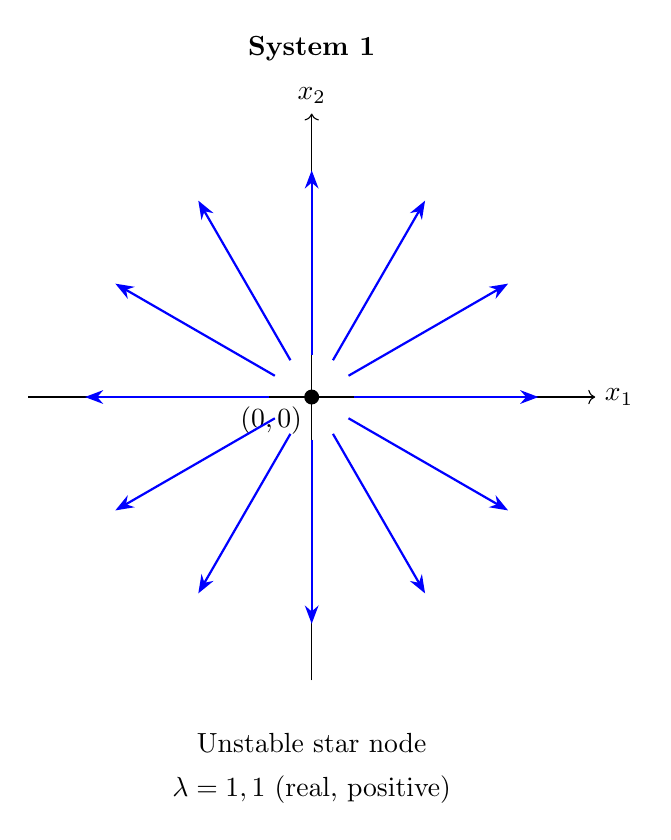
\begin{tikzpicture}[scale=1.8]
% Axes
\draw[->] (-2,0) -- (2,0) node[right] {$x_1$};
\draw[->] (0,-2) -- (0,2) node[above] {$x_2$};

% Equilibrium
\fill (0,0) circle (1.5pt);
\node[below left] at (0,0) {$(0,0)$};

% Radial trajectories
\foreach \angle in {0,30,60,90,120,150,180,210,240,270,300,330} {
    \draw[->,thick,blue,>=Stealth] ({0.3*cos(\angle)},{0.3*sin(\angle)}) -- ({1.6*cos(\angle)},{1.6*sin(\angle)});
}

\node[above] at (0,2.3) {\textbf{System 1}};
\node[below] at (0,-2.3) {Unstable star node};
\node[below] at (0,-2.6) {$\lambda = 1, 1$ (real, positive)};
\end{tikzpicture}

\hspace{1cm}

\textbf{System 2: Unstable Focus}

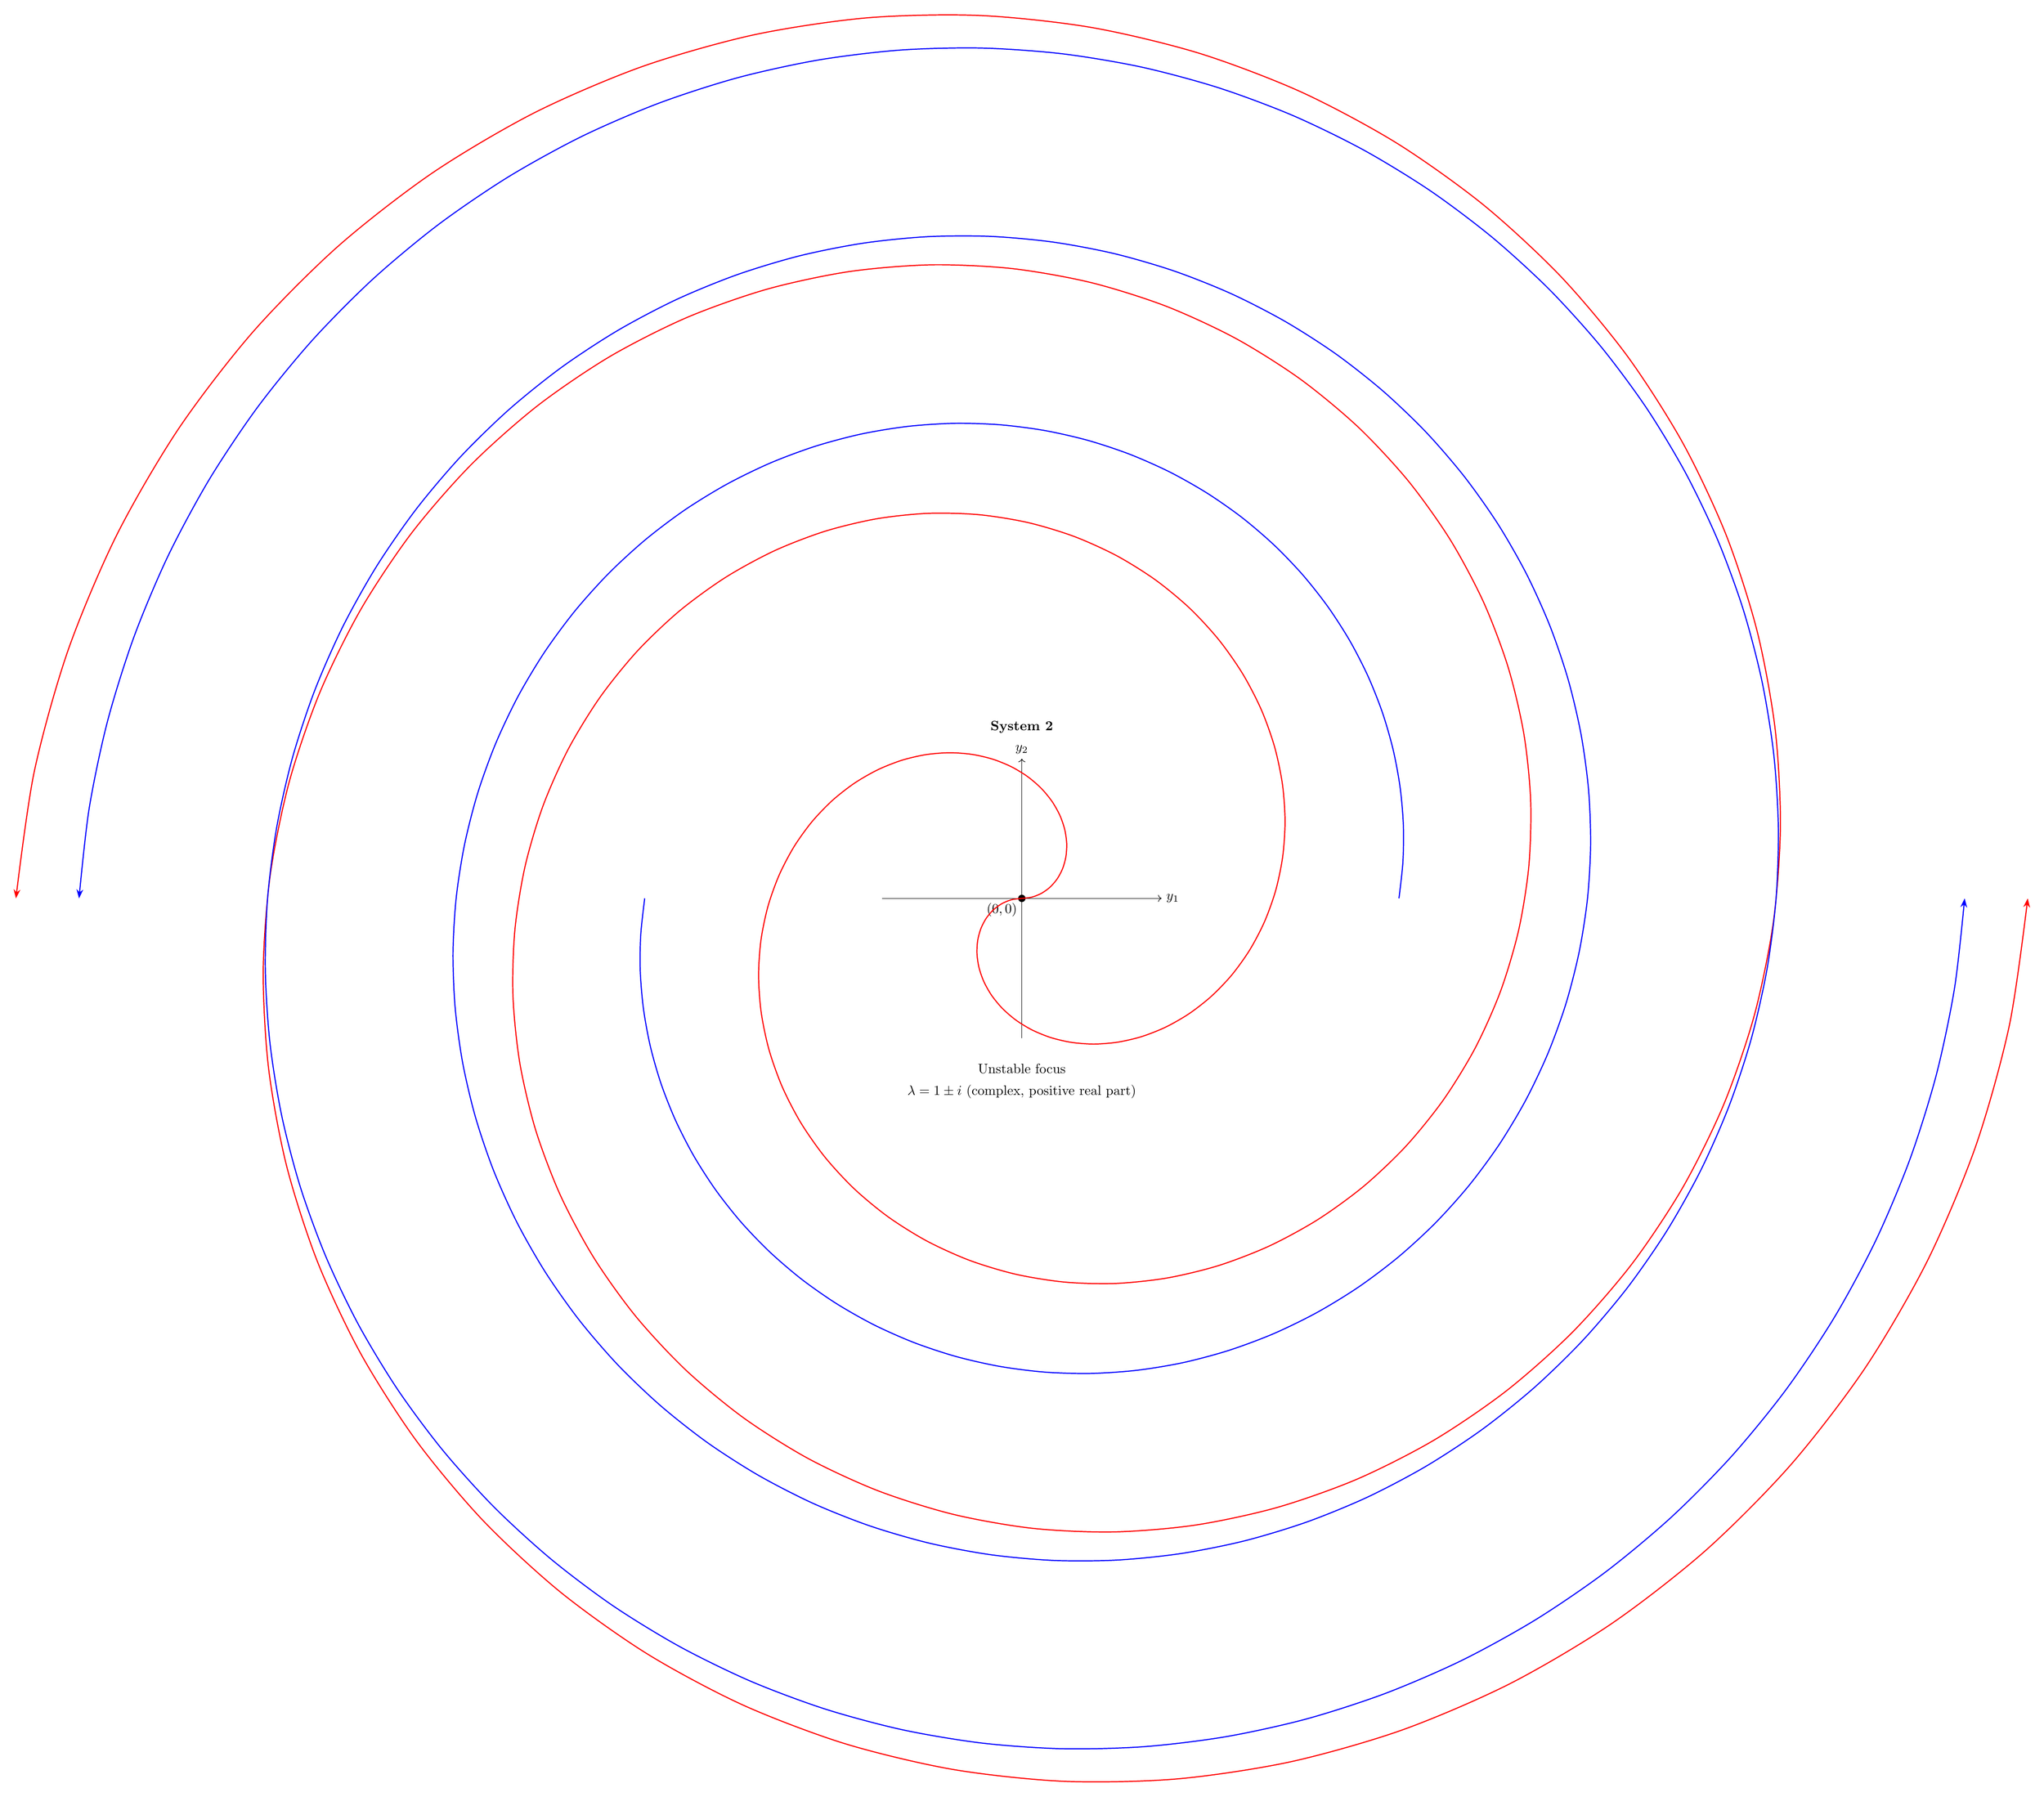
\begin{tikzpicture}[scale=1.8]
% Axes
\draw[->] (-2,0) -- (2,0) node[right] {$y_1$};
\draw[->] (0,-2) -- (0,2) node[above] {$y_2$};

% Equilibrium
\fill (0,0) circle (1.5pt);
\node[below left] at (0,0) {$(0,0)$};

% Spiral trajectories (outward)
\draw[thick,red,domain=0:720,smooth,samples=100,>=Stealth,->]
    plot ({0.02*\x*cos(\x)},{0.02*\x*sin(\x)});
\draw[thick,red,domain=0:720,smooth,samples=100,>=Stealth,->]
    plot ({-0.02*\x*cos(\x)},{-0.02*\x*sin(\x)});
\draw[thick,blue,domain=360:900,smooth,samples=100,>=Stealth,->]
    plot ({0.015*\x*cos(\x)},{0.015*\x*sin(\x)});
\draw[thick,blue,domain=360:900,smooth,samples=100,>=Stealth,->]
    plot ({-0.015*\x*cos(\x)},{-0.015*\x*sin(\x)});

\node[above] at (0,2.3) {\textbf{System 2}};
\node[below] at (0,-2.3) {Unstable focus};
\node[below] at (0,-2.6) {$\lambda = 1 \pm i$ (complex, positive real part)};
\end{tikzpicture}
\end{center}

\subsection*{Final Answer for Part (a)}

\begin{equation}
\boxed{
\begin{aligned}
&\textbf{System 1:} \text{ Unstable star node with radial trajectories} \\
&\textbf{System 2:} \text{ Unstable focus with outward spiraling trajectories}
\end{aligned}
}
\end{equation}

Both systems have unstable equilibria at the origin, but with qualitatively different trajectory structures.

\end{solution}

\vspace{10pt}
\hrule
\vspace{10pt}

\section{Question 6(b): Prove Topological Equivalence}

\begin{solution}

\subsection*{Overview of Proof Strategy}

\begin{itemize}[leftmargin=*]
\item \stage{STAGE X (Goal):} Show there exists a continuous, invertible map (homeomorphism) transforming trajectories of System 1 to System 2 while preserving time direction.

\item \stage{STAGE Y (Method):} From Lecture Notes (Section 11, page 37), topological equivalence means the systems have the same qualitative behavior. We'll use polar coordinates to reveal the underlying structure and construct an explicit homeomorphism.

\item \stage{STAGE Z (Steps):} Convert to polar, solve, construct map $h: (r, \theta) \mapsto (\rho, \phi)$, verify continuity and invertibility.
\end{itemize}

\subsection*{Part (i): System 1 in Polar Coordinates}

\textbf{Coordinate Transformation:}
\begin{equation}
x_1 = r\cos\theta, \quad x_2 = r\sin\theta
\end{equation}

\textbf{Time Derivatives:}
\begin{align}
\dot{x}_1 &= \dot{r}\cos\theta - r\dot{\theta}\sin\theta \\
\dot{x}_2 &= \dot{r}\sin\theta + r\dot{\theta}\cos\theta
\end{align}

\textbf{Substitute Original Equations} ($\dot{x}_1 = x_1$, $\dot{x}_2 = x_2$):
\begin{align}
r\cos\theta &= \dot{r}\cos\theta - r\dot{\theta}\sin\theta \label{eq:s1_1}\\
r\sin\theta &= \dot{r}\sin\theta + r\dot{\theta}\cos\theta \label{eq:s1_2}
\end{align}

\textbf{Find $\dot{r}$:} Multiply \eqref{eq:s1_1} by $\cos\theta$, \eqref{eq:s1_2} by $\sin\theta$, and add:
\begin{align}
r\cos^2\theta + r\sin^2\theta &= \dot{r}\cos^2\theta + \dot{r}\sin^2\theta \\
r &= \dot{r}
\end{align}

\textbf{Find $\dot{\theta}$:} Multiply \eqref{eq:s1_1} by $(-\sin\theta)$, \eqref{eq:s1_2} by $\cos\theta$, and add:
\begin{align}
-r\sin\theta\cos\theta + r\sin\theta\cos\theta &= -\dot{r}\sin\theta\cos\theta + r\dot{\theta}\sin^2\theta \\
&\quad + \dot{r}\sin\theta\cos\theta + r\dot{\theta}\cos^2\theta \\
0 &= r\dot{\theta}(\sin^2\theta + \cos^2\theta) = r\dot{\theta}
\end{align}

For $r \neq 0$: $\dot{\theta} = 0$.

\subsection*{Result for System 1:}

\begin{equation}
\boxed{\dot{r} = r, \quad \dot{\theta} = 0}
\end{equation}

\begin{explanation}[Interpretation]
\begin{itemize}
\item $\dot{r} = r$: Exponential radial growth
\item $\dot{\theta} = 0$: No angular motion
\item Confirms straight-line trajectories from origin
\end{itemize}
\end{explanation}

\end{solution}

\vspace{10pt}
\hrule
\vspace{10pt}

\begin{solution}[continued]

\subsection*{Part (iii): System 2 in Polar Coordinates}

\textbf{Coordinate Transformation:}
\begin{equation}
y_1 = \rho\cos\phi, \quad y_2 = \rho\sin\phi
\end{equation}

\textbf{Time Derivatives:}
\begin{align}
\dot{y}_1 &= \dot{\rho}\cos\phi - \rho\dot{\phi}\sin\phi \\
\dot{y}_2 &= \dot{\rho}\sin\phi + \rho\dot{\phi}\cos\phi
\end{align}

\textbf{Substitute Original Equations} ($\dot{y}_1 = y_1 - y_2$, $\dot{y}_2 = y_1 + y_2$):
\begin{align}
\rho\cos\phi - \rho\sin\phi &= \dot{\rho}\cos\phi - \rho\dot{\phi}\sin\phi \label{eq:s2_1}\\
\rho\cos\phi + \rho\sin\phi &= \dot{\rho}\sin\phi + \rho\dot{\phi}\cos\phi \label{eq:s2_2}
\end{align}

\textbf{Find $\dot{\rho}$:} Multiply \eqref{eq:s2_1} by $\cos\phi$, \eqref{eq:s2_2} by $\sin\phi$, and add:
\begin{align}
&\rho\cos^2\phi - \rho\sin\phi\cos\phi + \rho\sin\phi\cos\phi + \rho\sin^2\phi \\
&\quad = \dot{\rho}\cos^2\phi - \rho\dot{\phi}\sin\phi\cos\phi + \dot{\rho}\sin^2\phi + \rho\dot{\phi}\sin\phi\cos\phi \\
\rho(\cos^2\phi + \sin^2\phi) &= \dot{\rho}(\cos^2\phi + \sin^2\phi) \\
\rho &= \dot{\rho}
\end{align}

\textbf{Find $\dot{\phi}$:} Multiply \eqref{eq:s2_1} by $(-\sin\phi)$, \eqref{eq:s2_2} by $\cos\phi$, and add:
\begin{align}
&-\rho\sin\phi\cos\phi + \rho\sin^2\phi + \rho\cos^2\phi + \rho\sin\phi\cos\phi \\
&\quad = -\dot{\rho}\sin\phi\cos\phi + \rho\dot{\phi}\sin^2\phi + \dot{\rho}\sin\phi\cos\phi + \rho\dot{\phi}\cos^2\phi \\
\rho(\sin^2\phi + \cos^2\phi) &= \rho\dot{\phi}(\sin^2\phi + \cos^2\phi) \\
\rho &= \rho\dot{\phi}
\end{align}

For $\rho \neq 0$: $\dot{\phi} = 1$.

\subsection*{Result for System 2:}

\begin{equation}
\boxed{\dot{\rho} = \rho, \quad \dot{\phi} = 1}
\end{equation}

\begin{explanation}[Interpretation]
\begin{itemize}
\item $\dot{\rho} = \rho$: Same exponential radial growth as System 1
\item $\dot{\phi} = 1$: Constant angular velocity (rotation)
\item Produces spiral trajectories: exponential growth + rotation
\end{itemize}
\end{explanation}

\end{solution}

\vspace{10pt}
\hrule
\vspace{10pt}

\begin{solution}[continued]

\subsection*{Part (iv): Solve the Polar Systems}

\textbf{System 1: } $\dot{r} = r$, $\dot{\theta} = 0$

These are decoupled ODEs:

\textit{For $r(t)$:}
\begin{align}
\frac{dr}{dt} &= r \\
\frac{dr}{r} &= dt \\
\ln|r| &= t + C_1 \\
r(t) &= Ae^t
\end{align}

With initial condition $r(0) = r_0$: $A = r_0$, so:
\begin{equation}
r(t) = r_0 e^t
\end{equation}

\textit{For $\theta(t)$:}
\begin{align}
\frac{d\theta}{dt} &= 0 \\
\theta(t) &= \text{constant} = \theta_0
\end{align}

\textbf{Solution for System 1:}
\begin{equation}
\boxed{r(t) = r_0 e^t, \quad \theta(t) = \theta_0}
\end{equation}

\vspace{10pt}

\textbf{System 2: } $\dot{\rho} = \rho$, $\dot{\phi} = 1$

Again, decoupled ODEs:

\textit{For $\rho(t)$:}
\begin{align}
\frac{d\rho}{dt} &= \rho \\
\rho(t) &= \rho_0 e^t
\end{align}

\textit{For $\phi(t)$:}
\begin{align}
\frac{d\phi}{dt} &= 1 \\
\phi(t) &= t + \phi_0
\end{align}

\textbf{Solution for System 2:}
\begin{equation}
\boxed{\rho(t) = \rho_0 e^t, \quad \phi(t) = \phi_0 + t}
\end{equation}

\begin{explanation}[Comparing Solutions]
\textbf{System 1:}
\begin{itemize}
\item Radius grows exponentially: $r = r_0 e^t$
\item Angle fixed: $\theta = \theta_0$
\item Straight radial motion
\end{itemize}

\textbf{System 2:}
\begin{itemize}
\item Radius grows exponentially: $\rho = \rho_0 e^t$ (same rate!)
\item Angle increases linearly: $\phi = \phi_0 + t$
\item Spiral motion (exponential growth + rotation)
\end{itemize}

The radial growth is \textit{identical} - only the angular behavior differs!
\end{explanation}

\end{solution}

\vspace{10pt}
\hrule
\vspace{10pt}

\begin{solution}[continued]

\subsection*{Part (v): Construct the Homeomorphism}

We need to find a map that transforms solutions of System 1 into solutions of System 2.

\textbf{Proposed Homeomorphism:}
\begin{equation}
h: (r, \theta) \mapsto (\rho, \phi) \quad \text{where} \quad \begin{cases} \rho = r \\ \phi = \theta - \ln(r) \end{cases}
\end{equation}

\subsection*{Step 1: Verify the Map Transforms Solutions}

\textbf{Start with System 1 solution:} $r(t) = r_0 e^t$, $\theta(t) = \theta_0$

\textbf{Apply the map:}
\begin{align}
\rho(t) &= r(t) = r_0 e^t \\
\phi(t) &= \theta(t) - \ln(r(t)) = \theta_0 - \ln(r_0 e^t) = \theta_0 - \ln(r_0) - t
\end{align}

\textbf{Verify this satisfies System 2:}

Check $\dot{\rho} = \rho$:
\begin{equation}
\dot{\rho} = \frac{d}{dt}(r_0 e^t) = r_0 e^t = \rho \quad \checkmark
\end{equation}

Check $\dot{\phi} = 1$:
\begin{equation}
\dot{\phi} = \frac{d}{dt}(\theta_0 - \ln(r_0) - t) = 0 - 0 - 1 = -1 \quad \text{???}
\end{equation}

\textbf{Issue:} We get $\dot{\phi} = -1$, not $+1$. Let me reconsider the map.

\textbf{Corrected Homeomorphism:}
\begin{equation}
h: (r, \theta) \mapsto (\rho, \phi) \quad \text{where} \quad \begin{cases} \rho = r \\ \phi = \theta + \ln(r) \end{cases}
\end{equation}

\textbf{Apply the corrected map:}
\begin{align}
\rho(t) &= r(t) = r_0 e^t \\
\phi(t) &= \theta(t) + \ln(r(t)) = \theta_0 + \ln(r_0 e^t) = \theta_0 + \ln(r_0) + t
\end{align}

\textbf{Verify System 2:}

Check $\dot{\rho} = \rho$:
\begin{equation}
\dot{\rho} = r_0 e^t = \rho \quad \checkmark
\end{equation}

Check $\dot{\phi} = 1$:
\begin{equation}
\dot{\phi} = \frac{d}{dt}(\theta_0 + \ln(r_0) + t) = 0 + 0 + 1 = 1 \quad \checkmark
\end{equation}

Perfect! The corrected map works.

\subsection*{Step 2: Verify Homeomorphism Properties}

A homeomorphism must be:
\begin{enumerate}
\item Continuous
\item Bijective (one-to-one and onto)
\item Have continuous inverse
\end{enumerate}

\textbf{Forward Map:}
\begin{equation}
h(r, \theta) = (r, \theta + \ln r) = (\rho, \phi)
\end{equation}

\textbf{Inverse Map:}

From $\rho = r$ and $\phi = \theta + \ln r$:
\begin{align}
r &= \rho \\
\theta &= \phi - \ln \rho
\end{align}

So:
\begin{equation}
h^{-1}(\rho, \phi) = (\rho, \phi - \ln \rho) = (r, \theta)
\end{equation}

\textbf{Continuity Check:}

\begin{itemize}
\item $h$: The function $(r, \theta) \mapsto (r, \theta + \ln r)$ is continuous for $r > 0$ (logarithm continuous on positive reals).

\item $h^{-1}$: The function $(\rho, \phi) \mapsto (\rho, \phi - \ln \rho)$ is continuous for $\rho > 0$.
\end{itemize}

\textbf{Bijectivity:}

\begin{itemize}
\item \textit{Injective:} If $h(r_1, \theta_1) = h(r_2, \theta_2)$, then $(r_1, \theta_1 + \ln r_1) = (r_2, \theta_2 + \ln r_2)$. This implies $r_1 = r_2$ and $\theta_1 + \ln r_1 = \theta_2 + \ln r_2$, hence $\theta_1 = \theta_2$. So $h$ is injective.

\item \textit{Surjective:} For any $(\rho, \phi)$ with $\rho > 0$, we can find $(r, \theta) = (\rho, \phi - \ln \rho)$ such that $h(r, \theta) = (\rho, \phi)$. So $h$ is surjective.
\end{itemize}

Therefore, $h$ is a valid homeomorphism.

\subsection*{Step 3: Geometric Interpretation}

\begin{explanation}[What the Homeomorphism Does]
The map $h(r, \theta) = (r, \theta + \ln r)$ can be understood as:

\begin{itemize}
\item \textbf{Radial component unchanged:} $\rho = r$ (same distance from origin)

\item \textbf{Angular component modified:} $\phi = \theta + \ln r$ (angle adjusted by logarithm of radius)

\item \textbf{Effect on trajectories:}
\begin{itemize}
\item System 1: Straight line at fixed angle $\theta_0$, growing exponentially
\item After mapping: The angle becomes $\phi = \theta_0 + \ln(r_0 e^t) = \theta_0 + \ln r_0 + t$
\item This increases linearly with time - exactly what System 2 does!
\end{itemize}

\item \textbf{Physical picture:} The homeomorphism "unwinds" the radial motion of System 1 into the spiral motion of System 2 by adding an angle that depends logarithmically on the radius.
\end{itemize}

From Lecture Notes (Section 11, page 37): Topological equivalence preserves the qualitative structure. Both systems:
\begin{itemize}
\item Have unstable equilibrium at origin
\item All trajectories escape to infinity
\item No limit cycles or other attractors
\end{itemize}

The homeomorphism shows these systems are fundamentally "the same" topologically, even though one has straight trajectories and the other has spirals.
\end{explanation}

\subsection*{Final Answer for Part (b)}

\begin{equation}
\boxed{
\begin{aligned}
&\text{The homeomorphism } h: \mathbb{R}^2 \setminus \{0\} \to \mathbb{R}^2 \setminus \{0\} \text{ defined by:} \\
&\qquad h(r, \theta) = (r, \theta + \ln r) = (\rho, \phi) \\
&\text{transforms solutions of System 1 into solutions of System 2.} \\
&\text{This proves the systems are topologically equivalent.}
\end{aligned}
}
\end{equation}

\textbf{Summary of verification:}
\begin{itemize}
\item System 1 solution: $r(t) = r_0 e^t$, $\theta(t) = \theta_0$
\item After mapping: $\rho(t) = r_0 e^t$, $\phi(t) = \theta_0 + \ln r_0 + t$
\item This satisfies System 2: $\dot{\rho} = \rho$, $\dot{\phi} = 1$ \checkmark
\item $h$ is continuous, bijective, with continuous inverse \checkmark
\item Therefore: Systems are topologically equivalent \checkmark
\end{itemize}

\end{solution}

\vspace{10pt}
\hrule
\vspace{10pt}

\section*{Summary: Topological Equivalence and its Significance}

\subsection*{Key Results}

\begin{enumerate}[leftmargin=*]
\item \textbf{System 1} ($\dot{x}_1 = x_1$, $\dot{x}_2 = x_2$): Unstable star node with straight radial trajectories

\item \textbf{System 2} ($\dot{y}_1 = y_1 - y_2$, $\dot{y}_2 = y_1 + y_2$): Unstable focus with outward spiral trajectories

\item \textbf{Polar forms reveal similarity:}
\begin{itemize}
\item System 1: $\dot{r} = r$, $\dot{\theta} = 0$
\item System 2: $\dot{\rho} = \rho$, $\dot{\phi} = 1$
\item Same radial dynamics, different angular dynamics
\end{itemize}

\item \textbf{Homeomorphism:} $h(r, \theta) = (r, \theta + \ln r)$ continuously deforms one phase portrait into the other

\item \textbf{Topological equivalence:} Despite different geometric appearance, the systems have identical topological structure
\end{enumerate}

\subsection*{Connection to Lecture Notes}

From Section 11 (pages 37-39):

\begin{itemize}[leftmargin=*]
\item \textbf{Hartman-Grobman Theorem:} For hyperbolic equilibria, nonlinear systems are topologically equivalent to their linearizations

\item \textbf{Hyperbolicity matters:} Both systems have eigenvalues with positive real part (hyperbolic), enabling the topological equivalence

\item \textbf{Topological classification:} Systems are grouped by the number and type of eigenvalues:
\begin{itemize}
\item System 1: Two positive real eigenvalues $\Rightarrow$ unstable node
\item System 2: Complex pair with positive real part $\Rightarrow$ unstable focus
\item Both are "unstable" topologically (trajectories escape)
\end{itemize}

\item \textbf{Importance:} Topological equivalence is coarser than similarity but more robust - it persists under continuous deformations of the vector field
\end{itemize}

\subsection*{Physical Intuition}

The homeomorphism demonstrates that:
\begin{itemize}
\item Adding rotation to radial growth changes geometry but not topology
\item Continuous transformations can relate seemingly different dynamical behaviors
\item Qualitative features (stability, number of equilibria, existence of cycles) are topologically invariant
\end{itemize}

\end{document}
